%%%%%%%%%%%%%%%%%%%%%%%%%%%%%%%%%%%%%%%%%%%%%%%%%%%%%%%%%%%%%%%%%%%%%%%%%%%%%%%%%%%%%%%%%%%%%%
%%%%%%%%%%%%%%%%%%%%%%%%%%%%%%%%%%%%%%%%%%%%%%%%%%%%%%%%%%%%%%%%%%%%%%%%%%%%%%%%%%%%%%%%%%%%%%
%%%%%%%%%%% GPU
%%%%%%%%%%%%%%%%%%%%%%%%%%%%%%%%%%%%%%%%%%%%%%%%%%%%%%%%%%%%%%%%%%%%%%%%%%%%%%%%%%%%%%%%%%%%%%
%%%%%%%%%%%%%%%%%%%%%%%%%%%%%%%%%%%%%%%%%%%%%%%%%%%%%%%%%%%%%%%%%%%%%%%%%%%%%%%%%%%%%%%%%%%%%%


% \cleardoublepage
\chapter{Equalizer Equations}
\label{sec:eq_eq}

\section{Overview}
There are 3 different kinds of equalizers I run
1. the solving ones!!!  They are equations like Ax=b where I have A and b but I need x
2. the initialized then iterative ones. CMA is initialized with MMSE then runs as many times a possible
3. the multiply ones! the FDEs are a simple multiply in the frequency domain

\section{Equations}

\subsection{The Solving Equalizers}


\subsubsection{The Zero-Forcing Equalizer}
The ZF equalizer was studied in the PAQ Phase 1 Final Report in ~equation 324
\begin{equation}
\mathbf{c}_\text{ZF} = (\mathbf{H}^\dagger \mathbf{H})^{-1} \mathbf{H}^\dagger \mathbf{u}_{n_0}
\label{eq:c_ZF_pinv}
\end{equation}
where $\mathbf{c}_\text{ZF}$ is a $L_{eq} \times 1$ vector of equalizer coefficients computed to invert the channel estimate $\mathbf{h}$
and $\mathbf{u}_{n_0}$ is the desired channel impulse response centered on $n0 = N_1+L_1+1$
\begin{equation}
\mathbf{u}_{n_0} = \begin{bmatrix} 0 \\ \vdots \\ 0 \\ 1 \\ 0 \\ \vdots \\ 0 \end{bmatrix}
	\begin{matrix*}[l] \left. \vphantom{\begin{matrix} 0 \\ \vdots \\ 0 \end{matrix}} \right\}
		\text{$n_0-1$ zeros}
		\\ \\
		\left. \vphantom{\begin{matrix} 0 \\ \vdots \\ 0 \end{matrix}} \right\}
		\text{$N_1+N_2+L_1+L_2-n_0+1$ zeros}
		\end{matrix*}.
		\label{eq:un0_ZF}
\end{equation}
The $L_{eq}+N_1+N_2 \times L_{eq}$ convolution matrix $\mathbf{H}$ is built using the channel estimate $\mathbf{h}$
\begin{equation}
\mathbf{H} = 
		\begin{bmatrix}
		h(-N_1)		&  			& 		 	&  			\\
		h(-N_1+1) 	& h(-N_1)	& 		 	&  			\\
		\vdots	 	& \vdots	& \ddots 	&  			\\
		h(N_2)		& h(N_2-1) 	&  			& h(-N_1)  	\\
		 			& h(N_2) 	&  			& h(-N_1+1) \\
		 			&  	   		&  			& \vdots	\\
		 			&  	   		&  			& h(N_2)	\\
	\end{bmatrix}.
\end{equation}
The computation of the coefficients in Equation \eqref{eq:c_ZF_pinv} can be simplified in a couple of ways: First the matrix multiplication of $\mathbf{H}^\dagger$ and $\mathbf{H}$ is the autocorrelation matrix of the channel
\begin{equation}
\mathbf{R}_{h} = 
\mathbf{H}^\dagger \mathbf{H} = 
		\begin{bmatrix}
		r_{h}(0)		& r^\ast_{h}(1)	& \cdots 	& r^\ast_{h}(L_{eq}-1)  	\\
		r_{h}(1) 		& r_{h}(0)		& \cdots 	& r^\ast_{h}(L_{eq}-2)  	\\
		\vdots	 			& \vdots				& \ddots 	&  							\\
		r_{h}(L_{eq}-1)	& r_{h}(L_{eq}-2)	& \cdots	& r_{h}(0)  			
	\end{bmatrix}
	\label{eq:R_h}
\end{equation}
where
\begin{equation}
r_{h}(k) = \sum_{n=-N_1}^{N_2} h(n) h^\ast(n-k).
\end{equation}
Second the matrix vector multiplication of $\mathbf{H}^\dagger$ and $\mathbf{u}_{n_0}$ is simply the $n_0$th row of $\mathbf{H}^\dagger$ or the conjugated $n_0$th column of $\mathbf{H}$.
A new vector $\mathbf{h}_{n_0}$ is defined by
\begin{equation}
\mathbf{h}_{n_0} = \mathbf{H}^\dagger \mathbf{u}_{n_0} = 
\begin{bmatrix} h(L_1) \\ \vdots \\ h(0) \\ \vdots \\ h(-L_2)  \end{bmatrix}.
\label{eq:h_no}
\end{equation}
To simplify, Equations \eqref{eq:R_h} and \eqref{eq:h_no} are substituted into Equation \eqref{eq:c_ZF_pinv} resulting in 
\begin{equation}
\mathbf{c}_\text{ZF} = \mathbf{R}^{-1}_{h} \mathbf{h}_{n_0}.
\label{eq:c_ZF_R_h}
\end{equation}

Computing the inverse of $\mathbf{R}_{h}$ is computationally heavy because an inverse is an $N^3$ operation.
To avoid an inverse, $\mathbf{R}_{h}$ is moved to the left side and $\mathbf{c}_\text{ZF}$ is found by solving a system of linear equations. 
Note that $r_{h}(k)$ only has support on $-L_{ch} \leq k \leq L_{ch}$ making $\mathbf{R}_{h}$ sparse or $\%63$ zeros.
The sparseness of $\mathbf{R}_{h}$ is leveraged to reduce computation drastically.
The Zero-Forcing Equalizer coefficients are computed by solving
\begin{equation}
\mathbf{R}_h \mathbf{c}_\text{ZF} = \mathbf{h}_{n_0}.
\label{eq:c_ZF_solve}
\end{equation}


\subsubsection{MMSE Equalizer}
The MMSE equalizer has the same form as the Zero-Forcing equalizer. 
The MMSE equalizer was also studied in the PAQ Phase 1 Final Report in ~equation 330.
\begin{equation}
\mathbf{c}_{MMSE} = \big[ \mathbf{G}\mathbf{G}^\dagger + \frac{\sigma_w^2}{\sigma_s^2}\mathbf{I}_{L_1+L_2+1} \big] \mathbf{g}^\dagger
\label{eq:MMSE_start}
\end{equation}
where
\begin{equation}
\mathbf{G} = 
		\begin{bmatrix}
		h(N_2)		& \cdots	& h(-N_1) 	&  			\\
					& h(N_2)	& \cdots 	& h(-N_1)	\\
				 	& 			& \ddots 	&  			& \ddots	\\
		 			&  	   		&  			& h(N_2)	& \cdots	& h(-N_1)	\\
	\end{bmatrix}
\end{equation}
and
\begin{equation}
\mathbf{g} = \begin{bmatrix} h(L_1) \cdots h(-L_2) \end{bmatrix}.
\end{equation}
The vector $\mathbf{g}^\dagger$ is also the same vector as $\mathbf{h}_{n_0}$ in Equation \eqref{eq:un0_ZF}.
The matrix multiplication $\mathbf{G}\mathbf{G}^\dagger$ is also the same autocorrelation matrix $\mathbf{R}_h$ as Equation \eqref{eq:R_h}.
The fraction $\frac{1}{2\hat{\sigma^2_w}}$ is substituted in for the fraction $\frac{\sigma_w^2}{\sigma_s^2}$ using Equation 333 Rice's report.
MMSE only differs from Zero-Forcing by adding the signal-to-noise ratio estimate down the diagonal of the autocorrelation matrix $\mathbf{R}_h$.
Substituting in all these similarities in to Equation \eqref{eq:MMSE_start} results in
\begin{equation}
\big[ \mathbf{R}_h + \frac{1}{2\hat{\sigma^2_w}} \mathbf{I}_{L_1+L_2+1} \big] \mathbf{c}_\text{MMSE} = \mathbf{h}_{n_0}.
\label{eq:c_MMSE_solve1}
\end{equation}
To further simplify the notation, $\mathbf{R}_{hw}$ is substituted in for $\mathbf{R}_h + \frac{1}{2\hat{\sigma^2_w}} \mathbf{I}_{L_1+L_2+1}$ where
\begin{equation}
\mathbf{R}_{hw} = 
\mathbf{R}_h + \frac{1}{2\hat{\sigma^2_w}} \mathbf{I}_{L_1+L_2+1} = 
		\begin{bmatrix}
		r_{h}(0) + \frac{1}{2\hat{\sigma^2_w}}	& r^\ast_{h}(1)							& \cdots 	& r^\ast_{h}(L_{eq}-1)  	\\
		r_{h}(1) 								& r_{h}(0) + \frac{1}{2\hat{\sigma^2_w}}& \cdots 	& r^\ast_{h}(L_{eq}-2)  	\\
		\vdots	 								& \vdots								& \ddots 	&  							\\
		r_{h}(L_{eq}-1)							& r_{h}(L_{eq}-2)						& \cdots	& r_{h}(0) + \frac{1}{2\hat{\sigma^2_w}}  			
	\end{bmatrix}.
	\label{eq:R_MMSE}
\end{equation}

The MMSE equalizer coefficients are solved for in a similar fashion to the Zero-Forcing equalizer coefficients in Equation \eqref{eq:c_ZF_solve}.
\begin{equation}
\mathbf{R}_{hw}\mathbf{c}_\text{MMSE} = \mathbf{h}_{n_0}.
\label{eq:c_MMSE_solve}
\end{equation}
\clearpage
\subsection{The Iterative Equalizer}

\subsubsection{The Constant Modulus Algorithm}
CMA uses a steepest decent algorithm.
\begin{equation}
\mathbf{c}_{b+1} = \mathbf{c}_{b}-\mu \nabla \mathbf{J}
\end{equation}
The vector $\mathbf{J}$ is the cost function and $\nabla J$ is the cost function gradient defined in the PAQ report 352 by
\begin{equation}
	\nabla J = \frac{2}{L_{pkt}} \sum_{n=0}^{L_{pkt}-1}
	\left[ \vphantom{\displaystyle\sum}  y(n) y^\ast(n) - R_2 \right]
	y(n)  \mathbf{r}^\ast(n).
\label{eq:DelJcma-approxr}
\end{equation}
where
\begin{equation}
\mathbf{r}(n) = \begin{bmatrix} r(n+L_1) \\ \vdots \\ r(n) \\ \vdots \\ r(n-L_2) \end{bmatrix}.
\end{equation}
This means $\nabla J$ is of the form
\begin{equation}
\nabla J = \begin{bmatrix} \nabla J(-L_1) \\ \vdots \\ \nabla J(0) \\ \vdots \\ \nabla J(L_2) \end{bmatrix}.
\end{equation}
To leverage the computational efficiency of the Fast Fourier Transform (FFT), Equation \eqref{eq:DelJcma-approxr} is re-expressed as a convolution.

To begin messaging $\nabla J$ 
\begin{equation}
z(n) = 	2\left[ \vphantom{\displaystyle\sum}  y(n) y^\ast(n) - R_2 \right] y(n)
\end{equation} 
is defined to make the expression of $\nabla J$ to be
\begin{equation}
	\nabla J = \frac{1}{L_{pkt}} \sum_{n=0}^{L_{pkt}-1}
	z(n)  \mathbf{r}^\ast(n).
\label{eq:DelJcma-midMassage}
\end{equation}
then writing the summation out in vector form
\begin{multline}
\nabla J
	= 
	\frac{z(0)}{L_{pkt}}
		\begin{bmatrix} r^\ast(L_1) \\ \vdots \\ r^\ast(0) \\ \vdots \\ r^\ast(L_2) \end{bmatrix} +
	\frac{z(1)}{L_{pkt}}
		\begin{bmatrix} r^\ast(1+L_1) \\ \vdots \\ r^\ast(1) \\ \vdots \\ r^\ast(1-L_2) \end{bmatrix} + \cdots
	\frac{z(L_{pkt}-1)}{L_{pkt}}
		\begin{bmatrix} r^\ast(L_{pkt}-1+L_1) \\ \vdots \\ r^\ast(L_{pkt}-1) \\ \vdots \\ r^\ast(L_{pkt}-1-L_2) \end{bmatrix}
\label{eq:delJ_writeoutr}.
\end{multline}
The $k$th value of $\nabla J$ is
\begin{equation}
\nabla J(k) = \frac{1}{L_{pkt}} \sum^{L_{pkt}-1}_{m=0}  z(m) r^\ast(m-k), \quad -L_1 \leq k \leq L_2.
\end{equation}
The summation almost looks like a convolution.
To put the summation in convolution form, define
\begin{equation}
\rho(n) = r^\ast(n).
\end{equation}
Now
\begin{equation}
\nabla J(k) = \frac{1}{L_{pkt}} \sum^{L_{pkt}-1}_{m=0}  z(m) \rho(k-m).
\label{eq:CMA_delJ_rice_reformed}
\end{equation}
Because $z(n)$ has support on $0 \leq n \leq L_{pkt}-1$ and $\rho(n)$ has support on $-L_{pkt}+1 \leq n \leq 0$, 
the result of the convolution sum $b(n)$ has support on $-L_{pkt}+1 \leq n \leq L_{pkt}-1$.
Putting all the pieces together, we have
\begin{align}
b(n) &= \sum^{L_{pkt}-1}_{m=0} z(m) \rho(n-m) \nonumber \\
	 &= \sum^{L_{pkt}-1}_{m=0} z(m) r^\ast(m-n)
	 \label{eq:CMA_conv_z_rho}
\end{align}
Comparing Equation \eqref{eq:CMA_delJ_rice_reformed} and \eqref{eq:CMA_conv_z_rho} shows that 
\begin{equation}
\nabla J(k) = \frac{1}{L_{pkt}} b(k), \quad -L_1 \leq k \leq L_2.
\label{eq:CMA_delJ_donzo}
\end{equation}
The values of interest are shown in Figure Foo!!!!(c)

This suggest the following algorithm for computing the gradient vector $\nabla J$
Matlab Code!!!

\clearpage
\subsection{The Multiply Equalizers}

\subsubsection{The Frequency Domain Equalizer One}
The Frequency Domain Equalizer One (FDE1) is the MMSE or wiener filter applied in the frequency domain.
Ian E. Williams and M. Saquib derived FDE1 for this project in a paper called Linear Frequency Domain Equalization of SOQPSK-TG for Wideband Aeronautical Telemetry.
The FDE1 equalizer is defined in Equation (11) as
\begin{equation}
C_\text{FDE1}(\omega) = \frac{\hat{H}^\ast(\omega)}{|\hat{H}(\omega)|^2+\frac{1}{\hat{\sigma}^2}}
\label{eq:FDE1}
\end{equation}
The term $C_\text{FDE1}(\omega)$ is the Frequency Domain Equalizer One frequency response at $\omega$.
The term $\hat{H}(\omega)$ is the channel estimate frequency response at $\omega$.
The term $\hat{\sigma}^2$ is the noise variance estimate, this term is completely independent of frequency because the noise is assumed to be white or spectrally flat.

FDE1 needs no massaging because Equation \eqref{eq:FDE1} is easily implemented in the GPU and it is computationally efficient.

\subsubsection{The Frequency Domain Equalizer One}
The Frequency Domain Equalizer Two (FDE2) is the MMSE or wiener filter applied in the frequency domain.
Ian E. Williams and M. Saquib derived FDE1 for this project in a paper called Linear Frequency Domain Equalization of SOQPSK-TG for Wideband Aeronautical Telemetry.
The FDE2 equalizer is defined in Equation (12) as
\begin{equation}
C_\text{FDE2}(\omega) = \frac{\hat{H}^\ast(\omega)}{|\hat{H}(\omega)|^2+\frac{\Psi(\omega)}{\hat{\sigma}^2}}
\label{eq:FDE2}
\end{equation}
FDE2 almost identical to FDE1.
The only difference is term $\Psi(\omega)$ in the denominator. 
The term $\Psi(\omega)$ is the average spectrum of SPQOSK-TG shown in Figure \ref{fig:SOQPSK_spectrum}.
\begin{figure}
	\centering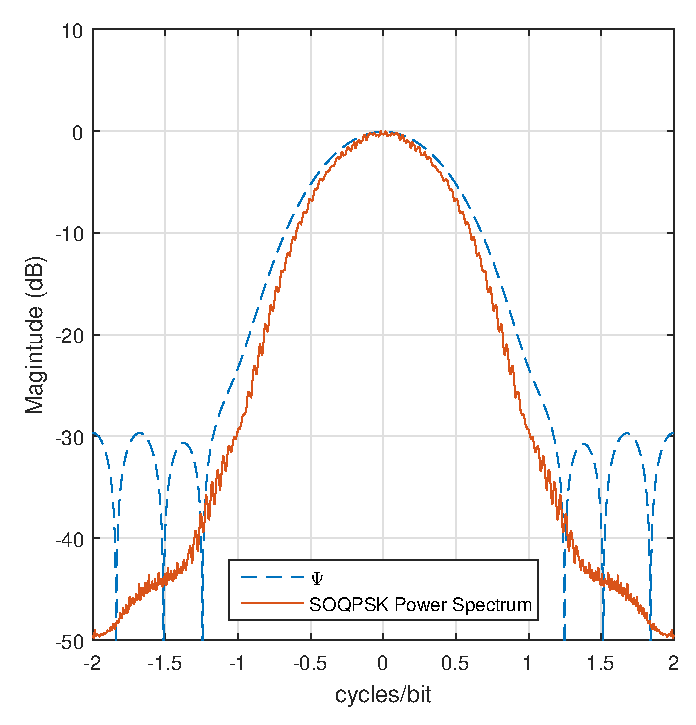
\includegraphics[width=5in]{figures/equations/FDE2_spectrum_PSI.eps}
	\caption{A block diagram illustrating organization of the algorithms in the GPU.}
	\label{fig:SOQPSK_spectrum}
\end{figure}
FDE2 needs no massaging because Equation \eqref{eq:FDE2} is easily implemented in the GPU and is computationally efficient.